\begin{figure}
\centering
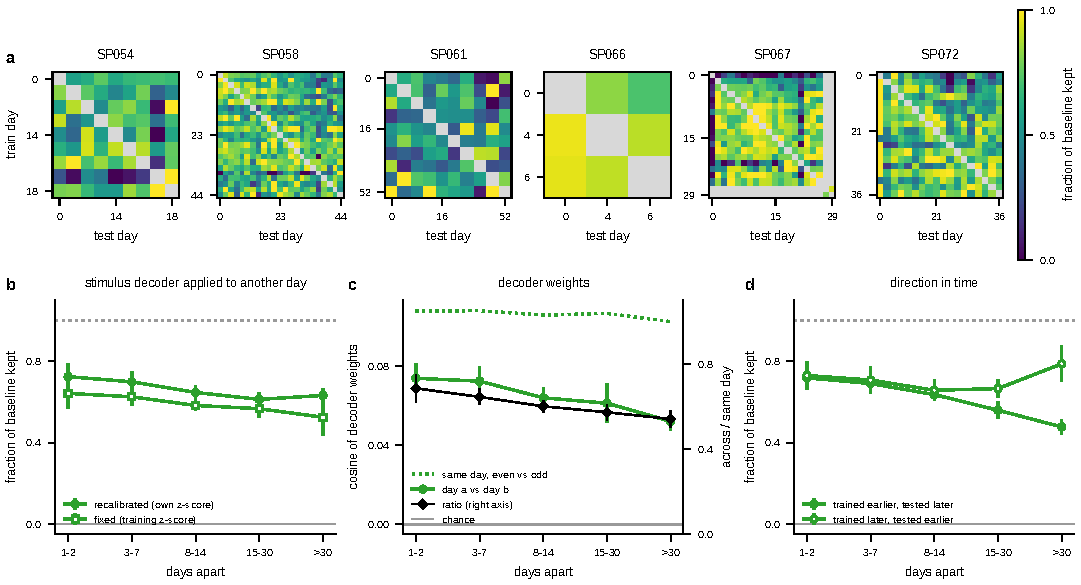
\includegraphics[width=\textwidth]{decoder_drift.pdf}
\caption{\textbf{How the stimulus decoder changes across days.} Stimulus-side ridge decoders on the neurons tracked in both sessions of a pair. Line styles and colours as in Fig.~\ref{fig:main}: dotted, same-day baseline; grey, chance; error bars, s.e.m.\ over mice.
\textbf{a}~Transfer matrices: decoder trained on day $i$ (rows) and tested on day $j$ (columns), as the fraction of the within-day accuracy kept (recalibrated). Axes: days since the first session (ticks at first, middle and last session). Grey: diagonal (baseline by definition) and pairs that did not meet the pair criteria (e.g.\ SP067's last two sessions, from a separate ROICaT run).
\textbf{b}~Fraction of baseline kept when the test data are z-scored with their own statistics (recalibrated, filled) or with those of the training half (fixed, open).
\textbf{c}~Cosine between decoder weight vectors fitted on the same day (even vs.\ odd half, dotted) and on two days (solid), and their ratio (black, right axis).
\textbf{d}~Transfer forward in time (trained on the earlier session, filled) and backward (trained on the later session, open). The difference is largely explained by later sessions having more trials (see text).}
\label{fig:drift}
\end{figure}
